\documentclass[11pt]{article}
\usepackage[utf8]{inputenc}
\usepackage{amsmath, amsfonts, amssymb}
\usepackage{graphicx}
\usepackage{geometry}
\usepackage{booktabs}
\usepackage{hyperref}
\usepackage{microtype}
\usepackage{xcolor} % TEMPORARY: marks Claude's additions in blue

\geometry{margin=1in}

\title{Homework Assignment 1: Slab-Geometry Boltzmann Equation}
\author{Tal Ramot}
\date{\today}

\begin{document}

\maketitle
\section*{Question 1 - Useful identity for the solution of the time-dependent slab-geometry Boltzmann equation}
In this question we are asked to prove the following identity:
\begin{equation}
    \psi(x,\mu,t;c) = ce^{-(1-c){v\Sigma_t} t}\psi(cx,\mu,ct;1) \label{eq:identity}
\end{equation}
We will do it in two parts. First, we will write down the equation that $\tilde{\psi} = \psi(cx,\mu,ct;1)$ satisfies, and then we will use it in order to prove that the product $ce^{-(1-c){v\Sigma_t} t}\tilde{\psi}$ satisfies the same equation as $\psi(x,\mu,t;c)$.
\subsection*{The equation for $\tilde{\psi}$}
\paragraph{Notation:} We will denote by $\Psi(X,\mu,T)\equiv\psi(X,\mu,T;1)$ the $c=1$ solution written in its own variables, and by $\Psi_T$ and $\Psi_X$ its partial derivatives with respect to them, so that $\tilde{\psi}(x,\mu,t) = \Psi(cx,\mu,ct)$ with $X=cx$ and $T=ct$. \textbf{This notation is used to avoid confusion when using the chain rule, as will be done immediately.}
First, $\Psi$ satisfies the $c=1$ equation in the variables $X$ and $T$:
\begin{equation}
    \frac{1}{v}\Psi_T + \mu \Psi_X + \Sigma_t \Psi = \frac{\Sigma_t}{2}\int_{-1}^{1} \Psi d\mu^\prime
\end{equation}
which after applying the chain rule, $\Psi_T = \frac{1}{c}\frac{\partial \tilde{\psi}}{\partial t}$ and $\Psi_X = \frac{1}{c}\frac{\partial \tilde{\psi}}{\partial x}$, and multiplying by $c$, becomes:
\begin{equation}
    \frac{1}{v}\frac{\partial \tilde{\psi}}{\partial t} + \mu \frac{\partial \tilde{\psi}}{\partial x} + c\Sigma_t \tilde{\psi} = \frac{c\Sigma_t}{2}\int_{-1}^{1} \tilde{\psi}d\mu^\prime \label{eq:tilde}
\end{equation}
So $\tilde{\psi}$ obeys the same equation as $\psi(x,\mu,t;c)$ except that it is removed at the rate $c\Sigma_t$ instead of $\Sigma_t$.
\subsection*{Proving the identity}
In this part we are going to simply subtitute the RHS of \ref{eq:identity} into the LHS of the equation for $\psi(x,\mu,t;c)$ and show that it satisfies the same equation. After substitution and application of the chain rule we get:
\begin{align}
    \text{LHS} &= \frac{1}{v}\left[c(c-1)v\Sigma_t e^{-(1-c)v\Sigma_t t}\tilde{\psi}+c\, e^{-(1-c)v\Sigma_t t}\frac{\partial\tilde{\psi}}{\partial t}\right] + \mu c\, e^{-(1-c)v\Sigma_t t}\frac{\partial\tilde{\psi}}{\partial x} + \Sigma_t c\, e^{-(1-c)v\Sigma_t t}\tilde{\psi} \\
    &= c e^{-(1-c)v\Sigma_t t}\left[\frac{1}{v}\frac{\partial\tilde{\psi}}{\partial t} + \mu \frac{\partial\tilde{\psi}}{\partial x} + \Sigma_t \tilde{\psi} + (c-1)\Sigma_t\tilde{\psi}\right] \\
    &= c e^{-(1-c)v\Sigma_t t}\left[\frac{1}{v}\frac{\partial\tilde{\psi}}{\partial t} + \mu \frac{\partial\tilde{\psi}}{\partial x} + c\Sigma_t \tilde{\psi}\right] \\
    &= c e^{-(1-c)v\Sigma_t t}\frac{c\Sigma_t}{2}\int_{-1}^{1} \tilde{\psi}d\mu^\prime = \frac{c\Sigma_t}{2}\int_{-1}^{1} c e^{-(1-c)v\Sigma_t t}\tilde{\psi}d\mu^\prime
\end{align}
where \ref{eq:tilde} was used in the last line, and this is exactly the RHS of the equation for $\psi(x,\mu,t;c)$.
\section*{Question 2 - Derivation of the time-dependent planar scalar flux for a plane source}
The relation between a plane source and a point source as studied in class is given by:
\begin{equation}
    \phi_{\text{pl}}(x) = 2\pi\int_{|x|}^{\infty} \phi_{\text{pt}}(r)rdr
\end{equation}
The solution taken from J. C. J. Paasschens is the point-source scalar flux $\phi_{\text{pt}}(r,t)$ for $c=1$, and therefore the planar-source scalar flux is given by the integration given above.
\begin{align}
    \phi_{\text{pl}}(x,t) &= 2\pi \int_{|x|}^{\infty} \frac{e^{-v\Sigma_t t}}{{4\pi r^2}}\delta(r-vt)rdr + {2\pi}\int_{|x|}^{\infty} \frac{{\left(1-r^2/v^2t^2\right)}^{1/8}}{\left(4\pi vt/(3\Sigma_t)\right)^{3/2}} e^{-v\Sigma_t t}G\left(v\Sigma_t t\left[1-\frac{r^2}{v^2t^2}\right]^{3/4}\right)\Theta(vt-r)rdr \\
    &= \frac{e^{-v\Sigma_t t}}{2vt}\Theta(vt-|x|) + \Theta(vt-|x|) \frac{2\pi e^{-v\Sigma_t t}}{\left(4\pi vt/(3\Sigma_t)\right)^{3/2}} \int_{|x|}^{vt} \left(1-\frac{r^2}{v^2t^2}\right)^{1/8} G\left(v\Sigma_t t\left[1-\frac{r^2}{v^2t^2}\right]^{3/4}\right)rdr \\
    &\overset{{\xi = r/vt}}{=} \frac{e^{-v\Sigma_t t}}{2vt}\Theta(vt-|x|) + \Theta(vt-|x|) \frac{2\pi e^{-v\Sigma_t t}(vt)^{1/2}}{\left(4\pi /(3\Sigma_t)\right)^{3/2}} \int_{\frac{|x|}{vt}}^{1} \left(1-\xi^2\right)^{1/8} G\left(a\left[1-\xi^2\right]^{3/4}\right) \xi d\xi \\
    &\overset{\substack{u=1-\xi^2\\ w=au^{3/4}}}{=} \frac{e^{-v\Sigma_t t}}{2vt}\left[1 + \sqrt{\frac{3}{\pi}}\int_{0}^{w_0}\sqrt{w}G(w)dw\right]\Theta(vt-|x|)
\end{align}


with $w_0 = a\left(1-\frac{x^2}{(vt)^2}\right)^{3/4}$, the powers combining as $\frac{1}{6}+\frac{1}{3}=\frac{1}{2}$ and the $\Sigma_t$ dependence cancelling in the last step (I used the assistance of AI in this algebric derivation). Finally, with the interpolation formula of Paasschens, $G(w) = e^{w}\sqrt{1+b/w}$ with $b=2.026$, the integral has a closed form:
\begin{equation}
    \int_{0}^{w_0}e^{w}\sqrt{w+b}\,dw = e^{w_0}\sqrt{w_0+b} - \sqrt{b} - \frac{\sqrt{\pi}}{2}e^{-b}\left[\text{erfi}\left(\sqrt{w_0+b}\right)-\text{erfi}\left(\sqrt{b}\right)\right]
\end{equation}
which \textbf{closes the derivation of the planar-source scalar flux for $c=1$.}
Of course the relation proved in Q1 can be used to get the solution for $c\neq 1$ using a simple scaling and multiplication by an exponential factor of the solution for $c=1$.
\section*{Question 3 - Classical and asymptotic diffusion against the exact solution}
\subsection*{Derivation of the time-dependent diffusion Green's function}
\label{sec:derivation}
The time-dependent diffusion equation is:
\begin{equation}
    \frac{1}{v}\frac{\partial \phi}{\partial t} - D\frac{\partial^2 \phi}{\partial x^2} + \Sigma_a\phi = S(x,t) \label{eq:fluxform}
\end{equation}
Take $S = \delta(x)\delta(t)$ and multiply \eqref{eq:fluxform} by $v$:
\begin{equation}
    \frac{\partial \phi}{\partial t} - Dv\frac{\partial^2 \phi}{\partial x^2} + v\Sigma_a\phi = v\,\delta(x)\delta(t) \label{eq:vform}
\end{equation}

\paragraph{Step 1: the pulse source is an initial condition.} Integrate \eqref{eq:vform} over
$t\in(0^-,0^+)$. The diffusion and absorption terms are bounded and contribute nothing in the
limit, so only the time derivative survives:
\begin{equation}
    \phi(x,0^+) - \phi(x,0^-) = v\,\delta(x) \qquad\Longrightarrow\qquad \phi(x,0^+) = v\,\delta(x)
\end{equation}
since nothing precedes the pulse. For $t>0$ the equation is source-free, so the problem is now
a pure initial-value problem (this is the same trick as in Assignment 1, Question 2)

\paragraph{Step 2: absorption factors out exactly.} As performed in the course, substituting
$\phi(x,t) = e^{-v\Sigma_a t}\,u(x,t)$ into \eqref{eq:vform} for $t>0$, the $-v\Sigma_a u$
produced by the time derivative cancels the absorption term identically and leaves the pure
heat equation
\begin{equation}
    \frac{\partial u}{\partial t} = Dv\frac{\partial^2 u}{\partial x^2},
    \qquad u(x,0^+) = v\,\delta(x)
\end{equation}
Note this step is untouched by the sign of $1-c$: for $c>1$ the exponential grows instead of
decays, and nothing else changes.

\paragraph{Step 3: Fourier transform.} With
$\hat u(k,t) = \int_{-\infty}^{\infty} u(x,t)e^{-ikx}dx$, the spatial derivative becomes
multiplication by $-k^2$ and the PDE becomes an ordinary differential equation in $t$ for each
$k$ separately:
\begin{equation}
    \frac{d\hat u}{dt} = -Dvk^2\,\hat u, \qquad \hat u(k,0^+) = v
    \qquad\Longrightarrow\qquad
    \hat u(k,t) = v\,e^{-Dvk^2t}
\end{equation}
the initial value being $v$ because the transform of $v\delta(x)$ is the constant $v$ --- a
delta excites every wavenumber equally.

\paragraph{Step 4: invert.} Completing the square in the exponent,
$-Dvtk^2 + ikx = -Dvt\left(k - \frac{ix}{2Dvt}\right)^2 - \frac{x^2}{4Dvt}$, and using
$\int_{-\infty}^{\infty}e^{-\alpha k^2}dk = \sqrt{\pi/\alpha}$:
\begin{equation}
    u(x,t) = \frac{v}{2\pi}\int_{-\infty}^{\infty} e^{-Dvk^2t}e^{ikx}dk
           = \frac{v}{\sqrt{4\pi Dvt}}\,e^{-x^2/(4Dvt)}
\end{equation}
Restoring the factor from Step 2 gives the Green's function:
\begin{equation}
    \boxed{\;\phi_{\text{diff}}(x,t;c) = \frac{v\,e^{-(1-c)\Sigma_t v t}}{\sqrt{4\pi Dvt}}\,
    \exp\!\left(-\frac{x^2}{4Dvt}\right)\;}\label{eq:green}
\end{equation}
which in the units of this assignment, $\Sigma_t = v = 1$ and $D = D_0(c)$, is the form
implemented in \texttt{src/homework2/diffusion.py}:
\begin{equation}
    \boxed{\;\phi_{\text{diff}}(x,t;c) = \frac{e^{-(1-c)t}}{\sqrt{4\pi D_0(c)\,t}}\,e^{-x^2/(4D_0(c)t)}\;}
\end{equation}

{\color{blue}
\paragraph{A second route: Fourier in space, then Laplace in time.}\mbox{}\\
Define
\begin{equation}
    \hat{\phi}(k,t) = \int_{-\infty}^{\infty}\phi(x,t)\,e^{-ikx}dx,
    \qquad
    \tilde{\phi}(k,s) = \int_{0^-}^{\infty}\hat{\phi}(k,t)\,e^{-st}dt
\end{equation}
and apply both to \eqref{eq:vform} term by term, with $\phi(x,0^-) = 0$:
\begin{align}
    \frac{\partial \phi}{\partial t} &\;\longrightarrow\; s\,\tilde{\phi} - \hat{\phi}(k,0^-) = s\,\tilde{\phi} \\
    -Dv\frac{\partial^2 \phi}{\partial x^2} &\;\longrightarrow\; Dvk^2\,\tilde{\phi} \\
    v\Sigma_a\,\phi &\;\longrightarrow\; v\Sigma_a\,\tilde{\phi} \\
    v\,\delta(x)\delta(t) &\;\longrightarrow\; v
\end{align}
so that
\begin{gather}
    \left(s + Dvk^2 + v\Sigma_a\right)\tilde{\phi}(k,s) = v \\
    \tilde{\phi}(k,s) = \frac{v}{s + Dvk^2 + v\Sigma_a}
\end{gather}
a single simple pole at $s = -(Dvk^2 + v\Sigma_a)$, so with
$\mathcal{L}^{-1}\{(s+\alpha)^{-1}\} = e^{-\alpha t}$,
\begin{equation}
    \hat{\phi}(k,t) = v\,e^{-\left(Dvk^2 + v\Sigma_a\right)t}
\end{equation}
and the Fourier inversion completes the square exactly as in Step 4:
\begin{align}
    \phi(x,t) &= \frac{v}{2\pi}\int_{-\infty}^{\infty} e^{-\left(Dvk^2 + v\Sigma_a\right)t}e^{ikx}dk \\
    &= \frac{v\,e^{-v\Sigma_a t}}{2\pi}\,e^{-x^2/(4Dvt)}\int_{-\infty}^{\infty} e^{-Dvt\left(k - \frac{ix}{2Dvt}\right)^2}dk \\
    &= \frac{v\,e^{-v\Sigma_a t}}{2\pi}\,e^{-x^2/(4Dvt)}\sqrt{\frac{\pi}{Dvt}}
     = \frac{v\,e^{-v\Sigma_a t}}{\sqrt{4\pi Dvt}}\,e^{-x^2/(4Dvt)}
\end{align}
which is \eqref{eq:green}, with $\Sigma_a = (1-c)\Sigma_t$.
}

\subsection*{Parts 3(a) and 3(b): the comparison}
\label{sec:comparison}

Each figure fixes $c$ and shows $t = 1, 2, 3, 4, 7, 15$. The vertical line marks the causal
front $|x| = vt$, beyond which the exact solution is identically zero. Only $x \ge 0$ is
plotted; all three solutions are even in $x$.

\begin{figure}[h]
    \centering
    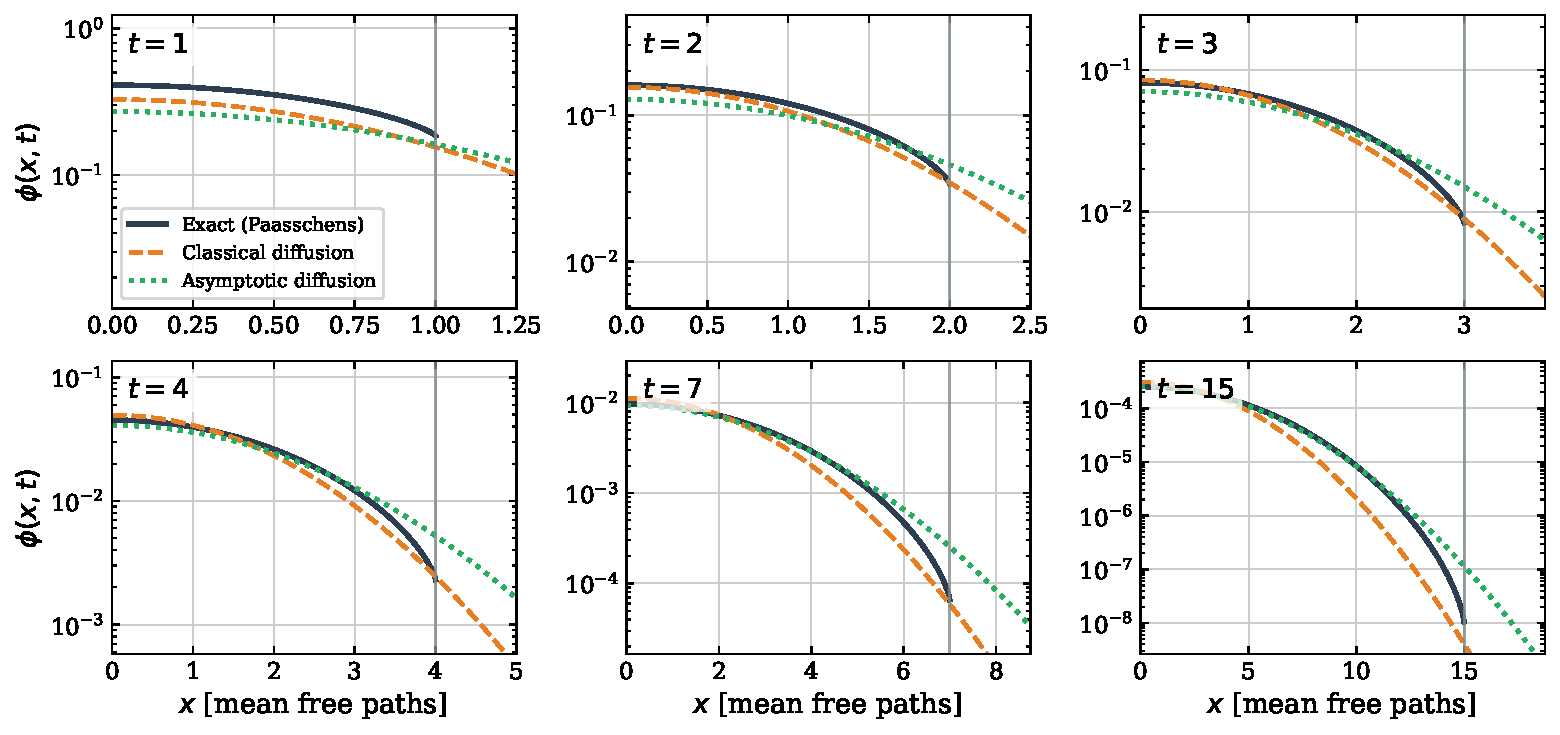
\includegraphics[width=\textwidth]{figs/q3_comparison_c0.6.pdf}
    \caption{$c = 0.6$.}
\end{figure}

\begin{figure}[h]
    \centering
    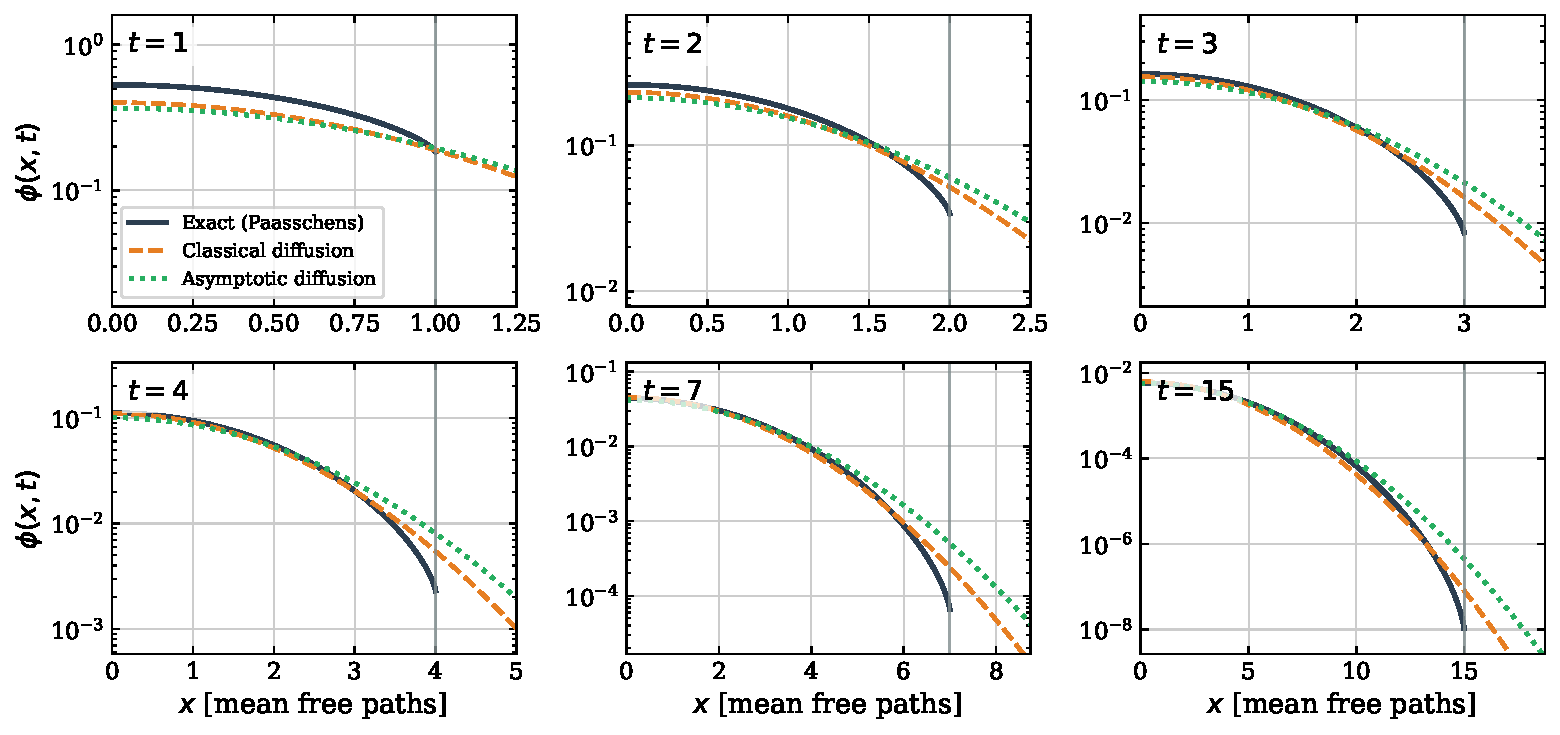
\includegraphics[width=\textwidth]{figs/q3_comparison_c0.8.pdf}
    \caption{$c = 0.8$.}
\end{figure}

\begin{figure}[h]
    \centering
    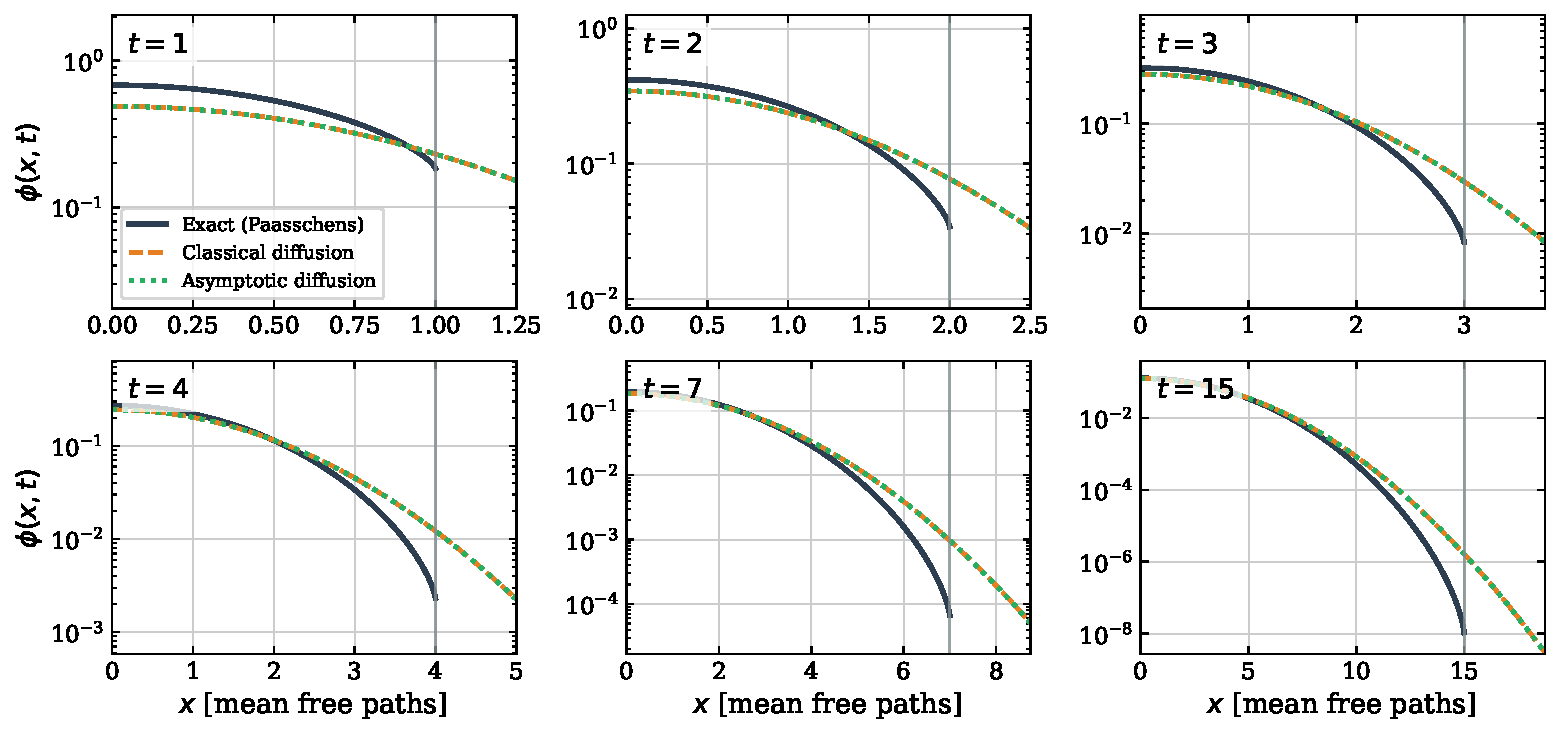
\includegraphics[width=\textwidth]{figs/q3_comparison_c1.pdf}
    \caption{$c = 1$. The two diffusion coefficients coincide at $D_0 = 1/3$, so the classical
    and asymptotic curves overlie each other.}
\end{figure}

\begin{figure}[h]
    \centering
    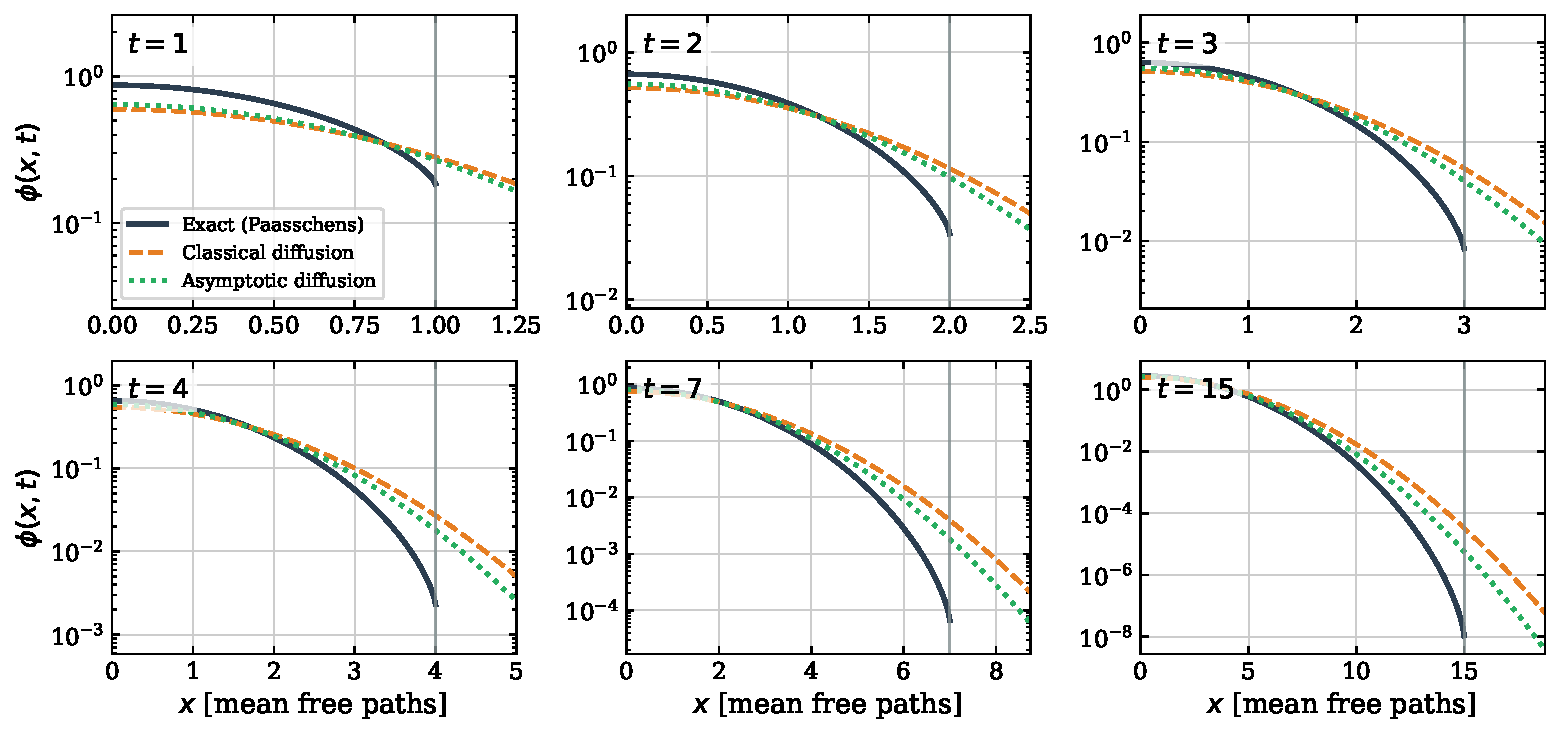
\includegraphics[width=\textwidth]{figs/q3_comparison_c1.2.pdf}
    \caption{$c = 1.2$.}
\end{figure}

\begin{figure}[h]
    \centering
    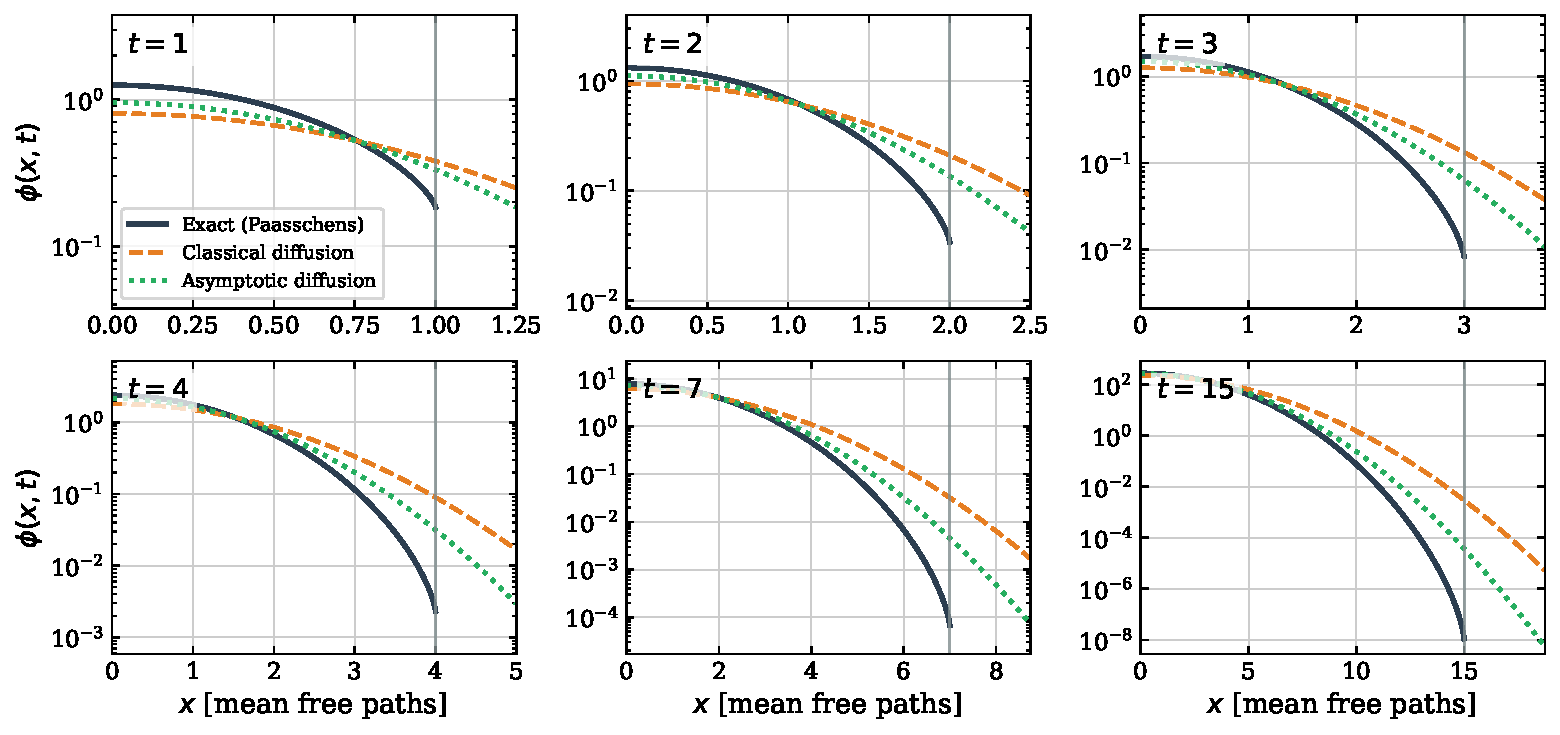
\includegraphics[width=\textwidth]{figs/q3_comparison_c1.5.pdf}
    \caption{$c = 1.5$.}
\end{figure}

\end{document}
